\begin{figure}
\centering
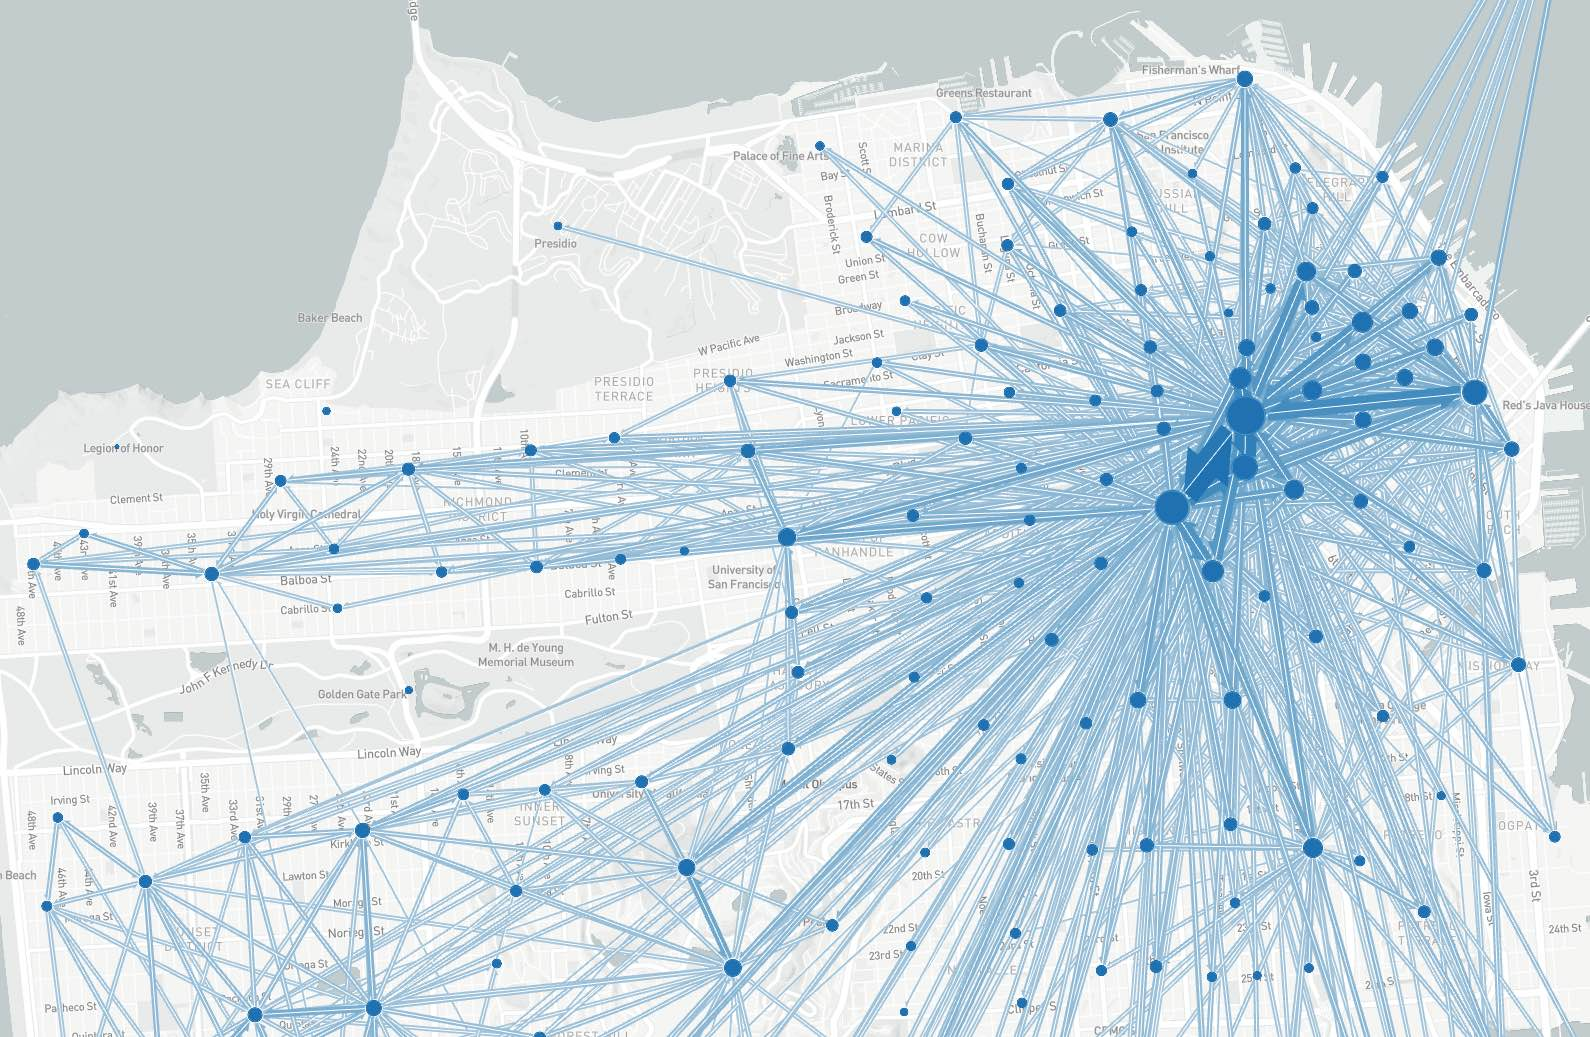
\includegraphics{assets/flow-map.jpg}
\caption{flow map example}
\end{figure}

\emph{A flow map of San Francisco}

Flowmaps depict \emph{aggregate movements} between origins and
destinations.

\hypertarget{usage}{%
\subsection{Usage}\label{usage}}

Flow maps can be included as panels in \textbf{Dashboards} or used as a
\textbf{standalone map}. See \href{dashboards}{Dashboard documentation}
for general tips on creating dashboard configurations.

\textbf{Standalone:} Create a \texttt{viz-flowmap*.yaml} file as
described below

-or-

\textbf{Embed in Dashboard:} \texttt{Create\ a\ dashboard-*.yaml} file
and include a \texttt{type:flowmap} section as desccribed below. - Each
chart panel is defined inside a \textbf{row} in a
\texttt{dashboard-*.yaml} file. - Standard title, description, height,
and width fields define the frame.

\begin{center}\rule{0.5\linewidth}{0.5pt}\end{center}

\hypertarget{configuration-reference-properties}{%
\subsubsection{Configuration reference
properties}\label{configuration-reference-properties}}

NOTE: These properties all go into a \texttt{viz-flowmap*.yaml} file
as-is, or, in a dashboard file they all go under the \texttt{props:}
section of a layout row. See the examples at the end of this document.

\hypertarget{general}{%
\paragraph{General}\label{general}}

\begin{itemize}
\tightlist
\item
  \textbf{title:} (optional) title of the visualization, appears right
  on top of the map. In the case of a dashboard: if a title is specified
  both under \texttt{general} and under \texttt{props}, the one under
  \texttt{general} will be used.
\item
  \textbf{description:} (optional) description of the visualization,
  appears between title and map. In the case of a dashboard: if a
  description is specified both under \texttt{general} and under
  \texttt{props}, the one under \texttt{general} will be used.
\end{itemize}

\hypertarget{data}{%
\paragraph{Data}\label{data}}

Two sets of data are needed: geographical data in the form of a .geojson
file and a .csv file containing the the flow data. The .geojson file can
contain polygons or points. To make a join between the .geojson file and
the .csv file possible, the feature IDs in the columns
\texttt{boundariesJoinCol}, \texttt{origin} and \texttt{destination}
need to match.

\begin{itemize}
\tightlist
\item
  \textbf{boundaries:} Geojson file with feature element boundaries.
\item
  \textbf{boundariesJoinCol:} The property in the boundary file
  containing the feature ID
\item
  \textbf{boundariesLabels:} The human readable name for the boundary ID
  column
\item
  \textbf{dataset:} CSV file containing at least three columns: origin,
  destination, and flow.
\item
  \textbf{origin:} The column name containing origin IDs
\item
  \textbf{destination:} The column name containing destination IDs
\item
  \textbf{flow:} The column name containing flow values
\end{itemize}

\hypertarget{general-map-settings}{%
\paragraph{General Map Settings}\label{general-map-settings}}

These settings are optional. Depending on the data used and the focus of
the work, adjustments may be helpful though.

\begin{itemize}
\tightlist
\item
  \textbf{center:} (optional) coordinates that the map centers on. Can
  be provided as array or string. If it is not provided, a center is
  calculated using a sample of the data.
\item
  \textbf{zoom:} (optional) zoom level of the map between 5 and 20. If
  it is not provided, the zoom level 9 is used.
\item
  \textbf{pitch:} (optional) If it is not provided, the pitch is 0.
\item
  \textbf{bearing:} (optional) If it is not provided, the bearing is 0.
\end{itemize}

\hypertarget{labels}{%
\paragraph{Labels}\label{labels}}

\begin{itemize}
\tightlist
\item
  \textbf{locationLabelsEnabled:} (optional) \texttt{true} or
  \texttt{false}. Turns the location labels on and off. If it is not
  provided, it is \texttt{true}.
\item
  \textbf{pickable:} (optional) \texttt{true} or \texttt{false}. When
  \texttt{true}, hovering over a flow highlights it. If it is not
  provided, it is \texttt{true}.
\end{itemize}

\hypertarget{flows}{%
\paragraph{Flows}\label{flows}}

\begin{itemize}
\tightlist
\item
  \textbf{animationEnabled:} (optional) \texttt{true} or \texttt{false}.
  Turns the animation of the flows on and off. If it is not provided, it
  is \texttt{true}.
\item
  \textbf{opacity:} (optional) value between \texttt{0} and \texttt{1},
  describes the opacity of the flows. If it is not provided, the opacity
  is \texttt{0}.
\end{itemize}

\hypertarget{clustering}{%
\paragraph{Clustering}\label{clustering}}

Unless otherwise specified clustering is turned on, meaning the flows
aggregate based on the zoom level. This is recommended for most
datasets. When vizualising smaller datasets, where there is less overlap
of the flows or trying to show specific details clustering can be turned
off and a specific clustering level can be used instead.

\begin{itemize}
\tightlist
\item
  \textbf{clusteringEnabled:} (optional) \texttt{true} or
  \texttt{false}. Turns the aggregation of the flows on and off. The
  standard value used is \texttt{true}.
\item
  \textbf{clusteringAuto:} (optional) \texttt{true}or \texttt{false}.
  Turns the automatic scaling of the clustering on and off. If turned
  off, a value for \textbf{clusteringLevel} should be provided. The
  standard value used is \texttt{true}.
\item
  \textbf{clusteringLevel:} (optional) The aggregation level of the
  flows. Relevant if \textbf{clusteringAuto} is \texttt{false}. Integers
  between 1 and 20.
\end{itemize}

\begin{center}\rule{0.5\linewidth}{0.5pt}\end{center}

\hypertarget{sample-dashboard.yaml-config-snippet}{%
\subsubsection{Sample dashboard.yaml config
snippet}\label{sample-dashboard.yaml-config-snippet}}

\begin{Shaded}
\begin{Highlighting}[]
\FunctionTok{layout}\KeywordTok{:}
\AttributeTok{  }\KeywordTok{{-}}\AttributeTok{ }\FunctionTok{title}\KeywordTok{:}\AttributeTok{ }\StringTok{\textquotesingle{}Trip Origin/Destination Flows\textquotesingle{}}
\AttributeTok{    }\FunctionTok{description}\KeywordTok{:}\AttributeTok{ }\StringTok{\textquotesingle{}Major flows shown\textquotesingle{}}
\AttributeTok{    }\FunctionTok{type}\KeywordTok{:}\AttributeTok{ }\StringTok{\textquotesingle{}flowmap\textquotesingle{}}
\AttributeTok{    }\FunctionTok{height}\KeywordTok{:}\AttributeTok{ }\DecValTok{10}
\AttributeTok{    }\FunctionTok{props}\KeywordTok{:}
\AttributeTok{      }\FunctionTok{boundaries}\KeywordTok{:}\AttributeTok{ }\StringTok{\textquotesingle{}taz1454.geojson\textquotesingle{}}
\AttributeTok{      }\FunctionTok{boundariesJoinCol}\KeywordTok{:}\AttributeTok{ }\StringTok{\textquotesingle{}TAZ1454\textquotesingle{}}
\AttributeTok{      }\FunctionTok{boundariesLabels}\KeywordTok{:}\AttributeTok{ }\StringTok{\textquotesingle{}TAZ\textquotesingle{}}
\AttributeTok{      }\FunctionTok{dataset}\KeywordTok{:}\AttributeTok{ }\StringTok{\textquotesingle{}trip{-}od{-}flows.csv\textquotesingle{}}
\AttributeTok{      }\FunctionTok{origin}\KeywordTok{:}\AttributeTok{ }\StringTok{\textquotesingle{}origin\textquotesingle{}}
\AttributeTok{      }\FunctionTok{destination}\KeywordTok{:}\AttributeTok{ }\StringTok{\textquotesingle{}destination\textquotesingle{}}
\AttributeTok{      }\FunctionTok{flow}\KeywordTok{:}\AttributeTok{ }\StringTok{\textquotesingle{}trips\textquotesingle{}}
\AttributeTok{      }\FunctionTok{animationEnabled}\KeywordTok{:}\AttributeTok{ }\CharTok{false}
\AttributeTok{      }\FunctionTok{clusteringEnabled}\KeywordTok{:}\AttributeTok{ }\CharTok{true}
\AttributeTok{      }\FunctionTok{clusteringAuto}\KeywordTok{:}\AttributeTok{ }\CharTok{true}
\AttributeTok{      }\FunctionTok{clusteringLevel}\KeywordTok{:}\AttributeTok{ }\DecValTok{20}
\AttributeTok{      }\FunctionTok{locationLabelsEnabled}\KeywordTok{:}\AttributeTok{ }\CharTok{true}
\AttributeTok{      }\FunctionTok{pickable}\KeywordTok{:}\AttributeTok{ }\CharTok{true}
\AttributeTok{      }\FunctionTok{opacity}\KeywordTok{:}\AttributeTok{ }\DecValTok{1}
\end{Highlighting}
\end{Shaded}

\hypertarget{sample-viz-flowmap.yaml-config-snippet}{%
\subsubsection{Sample viz-flowmap.yaml config
snippet}\label{sample-viz-flowmap.yaml-config-snippet}}

\begin{Shaded}
\begin{Highlighting}[]
\FunctionTok{title}\KeywordTok{:}\AttributeTok{ }\StringTok{\textquotesingle{}Trip Origin/Destination Flows\textquotesingle{}}
\FunctionTok{description}\KeywordTok{:}\AttributeTok{ }\StringTok{\textquotesingle{}Major flows shown\textquotesingle{}}
\FunctionTok{boundaries}\KeywordTok{:}\AttributeTok{ }\StringTok{\textquotesingle{}taz1454.geojson\textquotesingle{}}
\FunctionTok{boundariesJoinCol}\KeywordTok{:}\AttributeTok{ }\StringTok{\textquotesingle{}TAZ1454\textquotesingle{}}
\FunctionTok{boundariesLabels}\KeywordTok{:}\AttributeTok{ }\StringTok{\textquotesingle{}TAZ1454\textquotesingle{}}
\FunctionTok{dataset}\KeywordTok{:}\AttributeTok{ }\StringTok{\textquotesingle{}trip{-}od{-}flows.csv\textquotesingle{}}
\FunctionTok{origin}\KeywordTok{:}\AttributeTok{ }\StringTok{\textquotesingle{}origin\textquotesingle{}}
\FunctionTok{destination}\KeywordTok{:}\AttributeTok{ }\StringTok{\textquotesingle{}destination\textquotesingle{}}
\FunctionTok{flow}\KeywordTok{:}\AttributeTok{ }\StringTok{\textquotesingle{}trips\textquotesingle{}}
\FunctionTok{zoom}\KeywordTok{:}\AttributeTok{ }\DecValTok{9}
\FunctionTok{adaptiveScalesEnabled}\KeywordTok{:}\AttributeTok{ }\CharTok{true}
\FunctionTok{animationEnabled}\KeywordTok{:}\AttributeTok{ }\CharTok{true}
\FunctionTok{clusteringEnabled}\KeywordTok{:}\AttributeTok{ }\CharTok{true}
\FunctionTok{clusteringAuto}\KeywordTok{:}\AttributeTok{ }\CharTok{true}
\FunctionTok{clusteringLevel}\KeywordTok{:}\AttributeTok{ }\DecValTok{20}
\FunctionTok{locationLabelsEnabled}\KeywordTok{:}\AttributeTok{ }\CharTok{true}
\FunctionTok{pickable}\KeywordTok{:}\AttributeTok{ }\CharTok{true}
\FunctionTok{opacity}\KeywordTok{:}\AttributeTok{ }\DecValTok{1}
\end{Highlighting}
\end{Shaded}
